\documentclass{article}%
\usepackage[T1]{fontenc}%
\usepackage[utf8]{inputenc}%
\usepackage{lmodern}%
\usepackage{textcomp}%
\usepackage{lastpage}%
\usepackage{authblk}%
\usepackage{graphicx}%
%
\title{miR{-}1915 and miR{-}1225{-}5p Regulate the Expression of CD133, PAX2 and TLR2 in Adult Renal Progenitor Cells}%
\author{Samantha Gibson}%
\affil{Department of Cancer Biology and,}%
\date{01{-}01{-}2014}%
%
\begin{document}%
\normalsize%
\maketitle%
\section{Abstract}%
\label{sec:Abstract}%
What are the various, minute differences between RA{-}1A and C{-}21 or any colorectal tumor? These are determined by the mTORC1 protein, which is incorporated into colorectal tissue. Colorectal tumor and mTORC1 acts as precise control agents to destroy the epithelial cells surrounding epithelial and/or colon lining in these lesions.\newline%
Raab1A tumors can produce a range of molecules, and responses to these molecules indicate the presence of multiple types of tumors, including BRAF, FZ, GT1 and NFS2 as well as other mTORC1 antagonist and related agents. Different mTORC1 activators respond differently to tumors. Given that RA{-}1A tumors are more frequent than C{-}21, BRAF inhibitors are potentially warranted for RA in addition to being a potential adjuvant therapy for CRC tumors if these agents have full expression of the mTORC1 signature. Additional labels have also been developed to define mTORC1 as an adjuvant agent for CRC treatment.\newline%
Viruses targeting the mTORC1 target are common, and they can be found in nearly every tumor type and can affect healthy healthy tissues, including colon cancer cells. Viruses capable of shedding mTORC1, GL9 and other mTORC1 targets may interact with mTORC1 as a tumor antigen, which creates potential exposure to these mTORC1 agents.

%
\subsection{Image Analysis}%
\label{subsec:ImageAnalysis}%


\begin{figure}[h!]%
\centering%
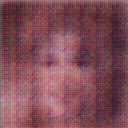
\includegraphics[width=150px]{500_fake_images/samples_5_285.png}%
\caption{A Black And White Photo Of A Person In A Mirror}%
\end{figure}

%
\end{document}